% This LaTeX was auto-generated from MATLAB code.
% To make changes, update the MATLAB code and export to LaTeX again.

\documentclass{article}

\usepackage[utf8]{inputenc}
\usepackage[T1]{fontenc}
\usepackage{lmodern}
\usepackage{graphicx}
\usepackage{color}
\usepackage{hyperref}
\usepackage{amsmath}
\usepackage{amsfonts}
\usepackage{epstopdf}
\usepackage[table]{xcolor}
\usepackage{matlab}

\sloppy
\epstopdfsetup{outdir=./}
\graphicspath{ {./parte4_images/} }

\begin{document}

\matlabtitle{III. Oferta laboral}


\vspace{1em}
\begin{par}
\begin{flushleft}
El mercardo de capitales y laboral están fuertemente relacionados (Ball, 1990). En este último apartado, abordaremos el problema del pescador desde la decisión que toma en el mercado laboral respecto al tiempo de uso en trabajar u ocio, decisión relevante que define sus niveles salariales disponibles para consumo.   Cada agente decide una combinación de horas de trabajo y ocio  que maximiza su nivel de satisfacción. Para los agentes que están trabajando, el costo de oportunidad de una hora adicional de ocio es el salario y la utilidad del agente es creciente en aumento de horas de ocio, pero a la vez si decide no trabajar piede salario para poder consumir por lo que disminuye la utilidad. En términos de la ecuación de Bellman podemos decir que el problema se escribe como
\end{flushleft}
\end{par}

\begin{par}
$$\begin{array}{l}
\max_{\left\lbrace a_{t+1} \;\;c_t \;{\;\;l}_{t\;} \;n_t \right\rbrace } \;V\left(a_t \right)=u\left(c_t \right)+\varphi \log \left(l\right)\;+\;\beta V_{t+1} \left(a_{t+1} \right)\\
s\ldotp a\;\;\;a_{t+1} =a_t \left(1+r\right)+{n\cdot w}_t -c_t \\
\;\;\;\;\;\;\;\;\;\;l_t +n_t =1\\
\;\;\;\;\;\;\;\;\;\;a_{t+1} \ge -h\\
\;\;\;\;\;\;\;\;\;\;c_t \;\ge 0\\
{\;\;\;\;\;\;\;\;\;1\ge \;l}_t \;,n_t \ge 0\\
\;\;\;\;\;\;\;\;\;\;\;a_1 =0\;;\\

\end{array}$$ 
\end{par}

\begin{par}
\begin{flushleft}
Al igual que en el apartado 1, trabajaremos con soluciones interiores, por lo que las restricciones de no negatividad y de esquema no ponzi no se resolverán algebráicamente en este apartado, sino que solo se incluirán en la resolución numérica (para más véase anexo donde se resuelve por método de KKT). Dicho esto, luego de la sustitución de la última restricción en la función de valor, obtenemos el siguiente Lagrangeano
\end{flushleft}
\end{par}

\begin{par}
$$L=\log \left(c_t \right)+\varphi \log \left(l\right)\;+\;\beta V_{t+1} \left(a_{t+1} \right)-\lambda \;\left(a_{t+1} -a_t \left(1+r\right)-{\left(1-l_t \right)\cdot w}_t +\;c_t \right)\;$$
\end{par}

\begin{par}
\begin{flushleft}
Las condiciones necesarias de primer orden, respecto a las variables de control
\end{flushleft}
\end{par}

\begin{par}
$$\begin{array}{l}
\frac{\partial }{\partial c_t }L=\frac{\partial u\left(c_t \right)}{\partial \;c_t }-\lambda =0\\
\frac{\partial }{\partial a_{t+1} }L=\beta \frac{\partial V_{t+1} \left(a_{t+1} \right)}{\partial \;a_{t+1} }-\lambda =0\\
\frac{\partial }{\partial l_t }L=\varphi \frac{\partial u\left(l_t \right)}{\partial l_t }-\lambda w_t =0
\end{array}$$
\end{par}

\begin{par}
\begin{flushleft}
Por consiguiente, las condiciones de optimalidad quedan escritas como
\end{flushleft}
\end{par}

\begin{par}
\begin{flushleft}
\textbf{(1) Condición de optimalidad del consumo}
\end{flushleft}
\end{par}

\begin{par}
$$\begin{array}{l}
\frac{\partial }{\partial c_t }L=\frac{\partial }{\partial c_t }u\left(c_t \right)=\beta \;\frac{\partial }{\partial c_t }V\left(a_{t+1} \right)\\
\frac{\partial }{\partial a_{t+1} }L=\beta \;\frac{\partial }{\partial a_{t+1} }V\left(a_{t+1} \right)
\end{array}$$
\end{par}

\begin{par}
\begin{flushleft}
Por teorema de la envolvente
\end{flushleft}
\end{par}

\begin{par}
$$\begin{array}{l}
\frac{\partial }{\partial a_{t+1} }V\left(a_{t+1} \right)\longrightarrow \frac{\partial }{\partial a_t }V\left(a_t \right)=\beta \;\frac{\partial }{\partial a_{t+1} }V\left(a_{t+1} \right)\cdot \left(1+r\right)\\
\;\;\;\;\;\;\;\;\;\;\;\;\;\;\;\;\;\;\;\;\;\;\;\;\;\;\;\;\;\;\;\;\;\;\frac{\partial }{\partial a_t }V\left(a_t \right)=\frac{\partial }{\partial c_t }u\left(c_t \right)\left(1+r\right)\\
\;\;\;\;\;\;\;\;\;\;\;\;\;\;\;\;\;\;\;\;\;\;\;\;\;\;\;\;\;\;\;\;\;\;\frac{\partial }{\partial a_{t+1} }V\left(a_{t+1} \right)=\frac{\partial }{\partial c_{t+1} }u\left(c_{t+1} \right)\cdot \left(1+r\right)
\end{array}$$
\end{par}

\begin{par}
\begin{flushleft}
Reemplazando por lo obtenido
\end{flushleft}
\end{par}

\begin{par}
$$\begin{array}{l}
\to \frac{\partial }{\partial c_t }u\left(c_t \right)=\beta \;\left(1+r\right)\;\frac{\partial }{\partial c_{t+1} }u\left(c_{t+1} \right)\\
c_t^{-1} =\beta \cdot \;\left(1+r\right)\cdot {c^{-1} }_{t+1} \;\;\;\;\;\;\;\;\;\\
c_{t+1} =\beta \left(1+r\right)\cdot c_t \;\;\;\;\;\;\;\;\;\;\;\;\;\;\;\;\;\;\;\;
\end{array}$$
\end{par}

\begin{par}
\begin{flushleft}
\textbf{(2) Condición de optimalidad del trabajo}
\end{flushleft}
\end{par}

\begin{par}
$$\varphi \frac{\partial u\left(l_t \right)}{\partial l_t }=\lambda w_t \;\;\;\;,\lambda =\;$$$$\frac{\partial u\left(c_t \right)}{\partial \;c_t }$$ 
\end{par}

\begin{par}
$$\begin{array}{l}
\frac{\partial u\left(c_t \right)}{\partial \;c_t }\cdot w_t =\varphi \frac{\partial u\left(l_t \right)}{\partial l_t }\\
\frac{w_t }{c_t }=\frac{\varphi }{l_t }\;\\
l_t =\frac{\varphi \cdot c_t }{w_t }
\end{array}$$
\end{par}

\begin{par}
\begin{flushleft}
Esta nueva condición que tenemos relaciona costo marginal de trabajar en términos del retorno marginal del ocio. Lo interesante de esta relación es que podemos a la vez ver dos efectos sobre la oferta laboral. El primero es el efecto sustitución, pues para un dado nivel de consumo  si sube el salario, el precio del ocio subirá respecto al consumo, por lo que subirá el tiempo dedicado al trabajo para poder consumir más. El segundo es el efecto ingreso pues si el salario sube, se tienen más dotaciones para subir consumo y tiempo en ocio, por lo que el agente disminuirá su tiempo dedicado al trabajo. La relevancia de $\varphi$ es que nos da la elasticidad del consumo respecto al salario, para entender la oferta laboral. 
\end{flushleft}
\end{par}

\begin{par}
\begin{flushleft}
Esta intuición económica que hemos dado la extenderemos a un análisis donde las restricciones de liquidez están activas y discutiremos el efecto que estas tienen sobre la oferta laboral.  
\end{flushleft}
\end{par}

\begin{par}
\begin{flushleft}
\textbf{Análisis sin restricciones de liquidez}
\end{flushleft}
\end{par}

\begin{par}
\begin{flushleft}
Para entender qué ocurre en el contexto con restricciones de liquidez, primero presentamos el escenario de la economía en ausencia de estas. En la Figura O presentamos la trayectoria de los agentes en un contexto de oferta laboral elástica, y donde la tasa de equilibrio es de aproximadamente 4,77\%, es decir $\beta \cdot R>1$. Así, el ciclo de vida del agente es coherente con lo que hemos discutido hasta ahora en este informe: el factor psicológico de impaciencia es menos preponderante que el factor económico del retorno por ahorrar hoy y consumir mañana, por lo que la trayectoria de consumo será creciente de \textit{t }a \textit{t+1. }Para suavizar consumo, el agente primero deberá pedir prestado activos, dado que en los primero periodos su salario es más bajo que el ingreso esperado (ingreso permanente). Ahora bien, a diferencia de los apartados anteriores, el cambio en los salarios si tiene un impacto sobre la oferta laboral como habíamos comentado antes (efecto sustitución e ingreso). 
\end{flushleft}
\end{par}

\begin{par}
\begin{flushleft}
El efecto total sobre la oferta laboral puede ser analizado a partir de la combinación de ambos efectos: la oferta laboral crece cuando el efecto sustitución  es mayor que el efecto ingreso, mientras que decrece cuando el efecto ingreso es mayor que el efecto sustitución. Como podemos notar, el efecto sustitución domina en la primera parte de la vida del agente, esto es, que cuando aumenta el salario el agente decide aumentar sus horas de trabajo para mantener sus niveles de consumo. Ahora bien, es incorrecto pensar que la disminución de la oferta laboral se da por el efecto ingreso pues eso implicaría que el valor del ocio excede el valor del salario en el mercado laboral. Lo bueno es que tenemos la última figura de la trayectoria salarial para evidenciar que los salarios no siguen subiendo cuando la oferta cae, sino que más bien este salario también empieza a decrecer. Esta primera descripción nos detalla una de las principales diferencias entre una oferta laboral inelástica (solo definida por parámetros exógenos y que es fija) y elástica (una que varía según la decisión óptima que enfrentan los agentes).
\end{flushleft}
\end{par}

\begin{par}
\begin{flushleft}
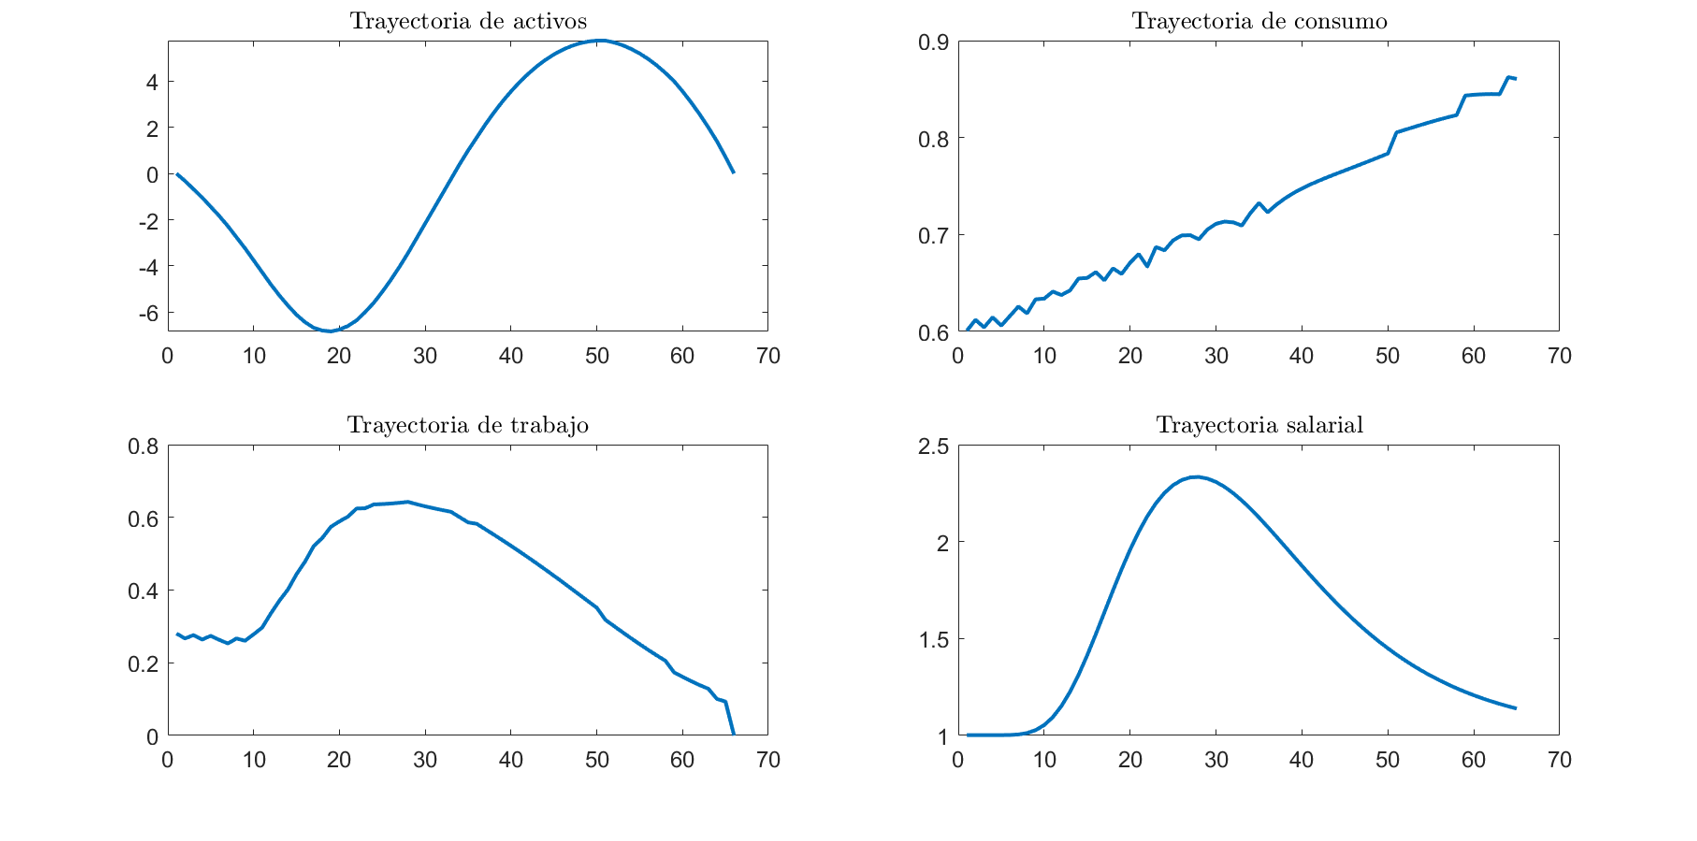
\includegraphics[width=\maxwidth{91.01856497742098em}]{image_0}
\end{flushleft}
\end{par}

\begin{par}
\begin{center}
Figura O. Trayectorias del agente sin restricciones
\end{center}
\end{par}

\begin{par}
\begin{flushleft}
Ahora bien, estas trayectorias pueden enfrentar escensarios más complejos de analizar en un contexto de restricciones crediticias. La razón: el consumo ya no estará \textit{dado }pues el acceso al credito afectará la posibilidad de suavizar el consumo por esta vía. Así, un canal presupuestario que puede seguir sustentando ese objetivo primordial del agente será la decisión por \textit{ocio }o \textit{consumo }(\textit{Consumption-Leisure Model Choice}). La Figura P
\end{flushleft}
\end{par}

\begin{par}
\begin{flushleft}
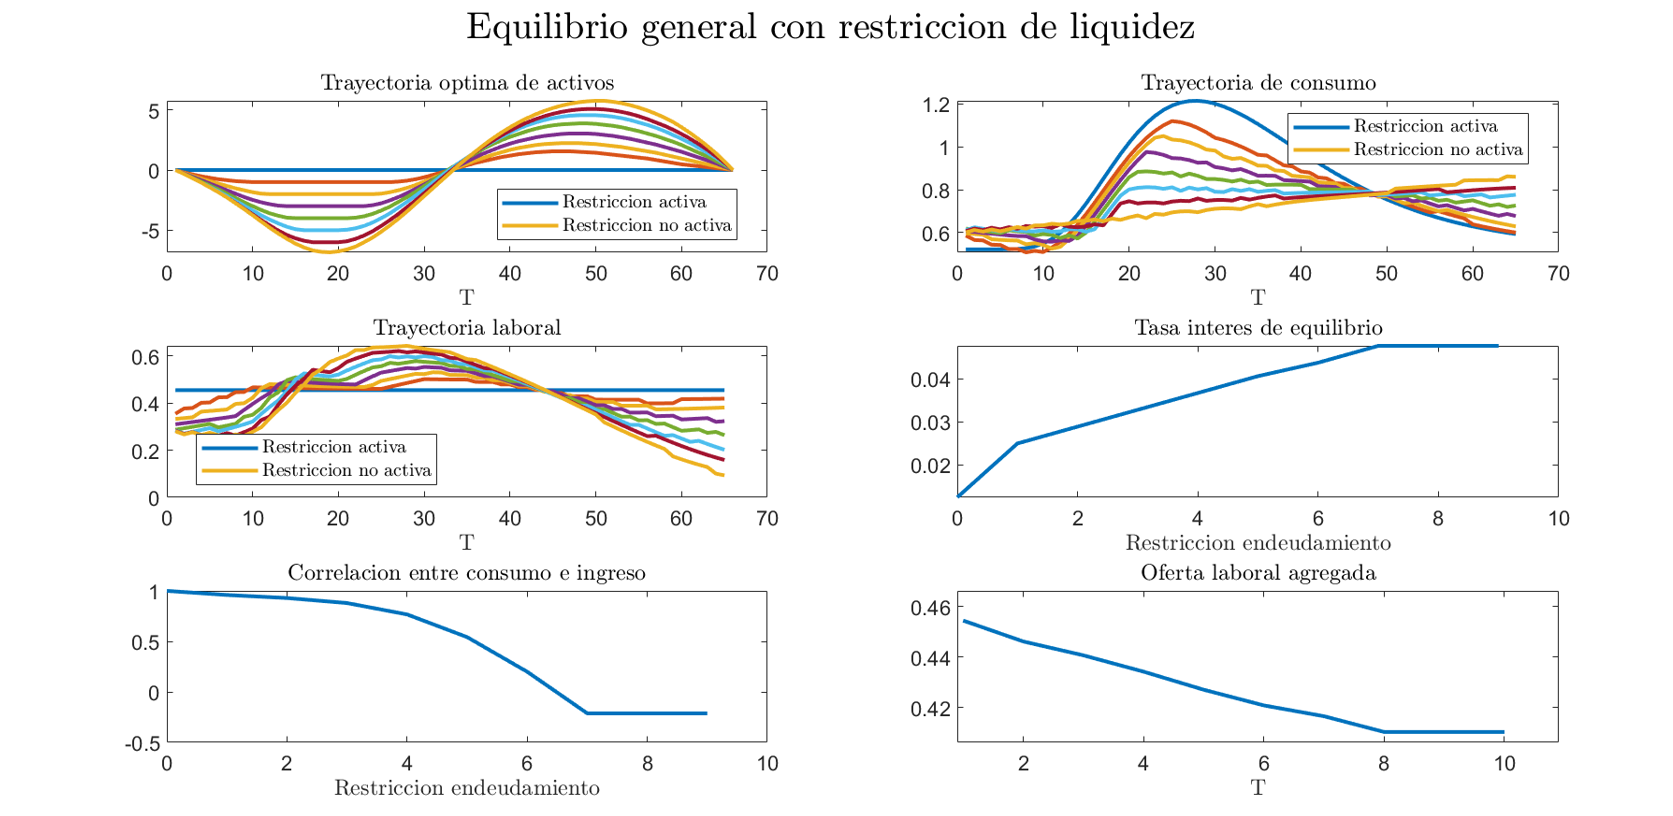
\includegraphics[width=\maxwidth{107.97792272955344em}]{image_1}
\end{flushleft}
\end{par}

\begin{par}
\begin{center}
Figura P. Equilibrio general en un contexto de fricciones financieras
\end{center}
\end{par}

\begin{par}
\begin{flushleft}
Recapitulemos el problema del agente. A diferencia de cuando la oferta laboral era inelástica la solución óptima del agente está sujeta no solo a la restricción presupuestaria sino que a la restricción temporal entre decidir usar tiempo en ocio o trabajo. Respecto a la primera restricción, el sujeto decide su consumo y ocio sujeto al precio del trabajo, haciendo sensible la trayectoria laboral no solo a los salarios (que en este caso además dependen de la tasa de interés \textit{r}) sino que también al acceso al credito. Si el agente está limitado en acceso al crédito o bien consume menos o bien aumenta sus horas laborales. Es por ello que en la discusión sobre el suavizamiento del consumo también es un actor relevante la relación entre el trabajo y la deuda. La hipótesis en genera es que la oferta laboral es fija, pero naturalmente podemos pensar que una hora adicional de trabajo puede representar una forma de soslayar la restricción crediticia y aumentar el bienestar.
\end{flushleft}
\end{par}

\begin{par}
\begin{flushleft}
Como podemos ver en la figura, en el equilibrio, el agente decide en este problema ajustar su nivel de consumo a la trayectoria salarial pero no reduciendo sus niveles, y más bien lo que hace es mantener sus niveles de horas laborales estables y \textit{nunca decrecientes}. De este modo, se mantienen los niveles de ingreso  estables para evitar efectos sobre el consumo. Ahora bien, esta intensidad en el trabajo no logra "revetir" o "netear" totalmente la restricción de liquidez. De ello se pueden desprender dos puntos. El primero es que, en un contexto con restricciones de liquidez y oferta laboral elástica la trayectoria del consumo se asimila a la trayectoria del salario, manteniéndose el análisis de correlación que hicimos en el segundo apartado. El segundo es que el agente en vez de aumentar aún más su tiempo dedicado en trabajo para acumular más riqueza para consumir, mantendrá sus niveles de empleo estables a lo largo de su ciclo de vida. 
\end{flushleft}
\end{par}

\begin{par}
\begin{flushleft}
Respecto a este último punto entra la discusión de la segunda restricción: la temporal. El agente puede usar su tiempo en ocio o trabajo ($l_t +n_t$ = 1). Si trabaja recibe salario para el consumo, que le otorga utilidad; pero si no trabaja ocupa su tiempo en ocio que también le da utilidad. Ese es el trade off principal. Y en particular, en un contexto de restricciones crediticias el agente tendrá una barrera para tratar de seguir suavizando su consumo en el tiempo y \textbf{a la vez }seguir satisfaciendo su necesidad de ocio. Así, en algunos casos el agente recibirá sus mayores niveles de utilidad cuando dedica todo al ocio, pues el costo de oportunidad del tiempo es relativamente alto y a la vez el salario es muy bajo. Entonces el agente decidirá salir de la fuerza de trabajo, lo que refiere a una solución esquina (Borjas, 2016). Esos casos son visibles al final del ciclo laboral del agente cuando la trayectoria laboral se va a cero, sobre todo en presencia de restricciones. Matemáticamente se da que la pendiente de la curva de indiferencia de trabajar cero horas corresponde al salario mínimo que está dispuesto a recibir el agente (\textit{reservation wage}), que es una representación teórica de cuanto el agente valora su tiempo usado en ocio. Ahora bien, en los casos en donde el agente incluso le gustaría ocupar más de su tiempo en ocio, hemos restringuido esas soluciones a no factibles, pero debemos destacar que estas si ocurrían cuando los agentes eran mucho mayores. La razón es que \textbf{los salarios tan bajos al final de su trayectoria de vida} y la \textbf{incapacidad de acceder a crédito}, hacían que el costo de consumir fuera mucho más alto que el de dejar de trabajar. Ocurre lo mismo en la primera etapa de la trayectoria de los jovenes pero sus niveles de consumo esperados son más bajos en equilibrio que en el caso de los adultos mayores. 
\end{flushleft}
\end{par}

\begin{par}
\begin{flushleft}
Fuera de este ejercicio de simulación, hemos revisado evidencia que también nos guía en un resultado de este estilo (Ball, 1990, Zeldes, 1989).Una investigación actual de Rossi y Trucchi (2016) revisan la relación entre las restricciones de liquidez y la oferta laboral, y lo que encuentran es que si bien efectivamente los agentes ajustan su intensidad en el trabajo (en término de horas dedicadas), el consumo también sufre modificaciones pero son menores.  Además, muestran que estas trayectorias varían según la edad y sexo de los agentes, lo que inspira a pensar que probablemente el costo de oportunidad de dejar de trabajar es mucho mayor para ciertos grupos que para otros. De hecho, un punto que destacan las autoras, y que se relaciona fielmente con lo que revisamos en Carroll (2001) tiene que ver con que para los jovenes el efecto de las restricciones financieras es realmente mucho menor (no se les restrigue tanto), y por ello mismo su oferta laboral no se ve tan afectada como en el caso de adultos en edad productiva o adultos mayores. 
\end{flushleft}
\end{par}

\matlabheading{Referencias}

\begin{par}
\begin{flushleft}
Ball, L. (1990). Intertemporal substitution and constraints on labor supply: evidence from panel data. \textit{Economic Inquiry}, \textit{28}(4), 706-724.
\end{flushleft}
\end{par}

\begin{par}
\begin{flushleft}
Borjas, G. J., \& Van Ours, J. C. (2016). \textit{Labor economics} (p. 45). Boston: McGraw-Hill/Irwin.
\end{flushleft}
\end{par}

\begin{par}
\begin{flushleft}
Rossi, M., \& Trucchi, S. (2016). Liquidity constraints and labor supply. \textit{European Economic Review}, \textit{87}, 176-193.
\end{flushleft}
\end{par}

\begin{par}
\begin{flushleft}
Zeldes, S. P. (1989). Consumption and liquidity constraints: an empirical investigation. \textit{Journal of political economy}, \textit{97}(2), 305-346.
\end{flushleft}
\end{par}

\matlabheading{\textbf{Anexos}}

\matlabheadingtwo{Consumo y ocio final}

\begin{par}
\begin{flushleft}
Para poder determinar el consumo y ocio final tomaremos la restricción presupuestaria (1) y temporal del agente (2). Además, por la restricción de \textit{no Ponzi }$a_{t+1} \;$ en el último periodo $T$ es cero.
\end{flushleft}
\end{par}

\begin{par}
$$\begin{array}{l}
a_{t+1} =a_t \;\left(1+r\right)+n\cdot \omega_t -c_{t\;\;\;\;\;\;\;\;\;\;\;\;\;\;\;} \left(1\right)\\
l_t +n_t =1\;\;\;\;\;\;\;\;\;\;\;\;\;\;\;\;\;\;\;\;\;\;\;\;\;\;\;\;\;\;\;\;\;\;\;\;\;\;\;\;\;\;\;\;\;\;\;\left(2\right)
\end{array}$$
\end{par}


\vspace{1em}
\begin{par}
$$\to c_t =a_t \left(1+r\right)+\left(1-l_t \right)\cdot \omega_t$$
\end{par}

\begin{par}
\begin{flushleft}
Además sabemos por la segunda condición de optimalidad del problema de maximización del agente que $l_t =\frac{\varphi \cdot c_t }{w_t }$
\end{flushleft}
\end{par}

\begin{par}
$$\begin{array}{l}
c_T =a_T \left(1+r\right)+\left(1-\frac{\varphi \cdot c_T }{w_T }\right)\cdot \omega_T \\
c_T =a_T \left(1+r\right)+\left(\omega_T -\varphi \cdot c_T \right)\\
c_T \;+\varphi \cdot c_T =a_T \left(1+r\right)+\omega_T \\
\left.c_T ={\left(a\right.}_T \left(1+r\right)+\omega_T \right)\cdot \frac{1}{1+\varphi }
\end{array}$$
\end{par}

\begin{par}
\begin{flushleft}
Por consiguiente podemos obtener $l_T$ (ocio en el último periodo)
\end{flushleft}
\end{par}

\begin{par}
$$\begin{array}{l}
\left.l_T =\left({\left(a\right.}_T \left(1+r\right)+\omega_T \right)\cdot \frac{1}{1+\varphi }\right)\cdot \frac{\varphi }{\omega_t }\\

\end{array}$$
\end{par}

\matlabheadingtwo{Policy ocio (Lpf) y consumo (Cpf)}

\begin{par}
\begin{flushleft}
Como podemos ver en la función labor.m Cpf se define como
\end{flushleft}
\end{par}

\begin{par}
$$\begin{array}{l}
c_t =a_t \left(1+r\right)+\left(1-l_t \right)\cdot \omega_t -a_{t+1} \\
c_t =a_t \left(1+r\right)+\left(1-\frac{\varphi \cdot c_t }{w_t }\right)\cdot \omega_t -a_{t+1} \\
c_t \;+\varphi \cdot c_t =a_t \left(1+r\right)+\omega_t -a_{t+1} \\
\left.{\mathrm{Cpf}\;\longmapsto \;c}_t ={\left(a\right.}_T \left(1+r\right)+\omega_T -a_{t+1} \right)\cdot \frac{1}{1+\varphi }
\end{array}$$
\end{par}

\begin{par}
\begin{flushleft}
Mientras que Lpf
\end{flushleft}
\end{par}

\begin{par}
$$\begin{array}{l}
l_t =\frac{c_{t\;} \cdot \varphi }{\omega_t }\\
\left.l_t =\left({\left(a\right.}_T \left(1+r\right)+\omega_T -a_{t+1} \right)\cdot \frac{1}{1+\varphi }\right)\cdot \frac{\varphi }{\omega_t }\\

\end{array}$$
\end{par}

\matlabheadingtwo{Restricciones con desigualdad}

\begin{par}
\begin{flushleft}
Este problema tenía un particular desafío respecto a cómo resolver en un contexto de restricciones con desigualdad. Para asegurar los resultados obtenidos, formalizaremos el problema del agente a partir del método de optimización de Karush-Kuhn-Tucker (KKT), para luego obtener dichas condiciones y traspasarlas a códigos en la función \href{./labor.m}{labor.m}
\end{flushleft}
\end{par}

\begin{par}
\begin{flushleft}
Cota inferior de la policy de activos 
\end{flushleft}
\end{par}

\begin{par}
$$\begin{array}{l}
c_t +a_{t+1} \;-\left(1-l_t \right)\cdot \omega_t =a_t \left(1+r\right)\\
a_t \left(1+r\right)=c_t +a_{t+1} \;-\omega_{t\;} +l_t \omega_t 
\end{array}$$
\end{par}

\begin{par}
\begin{flushleft}
El consumo y ocio es cero
\end{flushleft}
\end{par}

\begin{par}
$$\left.a_t ={\left(a\right.}_{t+1} \;-\omega_{t\;} \right)\cdot \left(\frac{1}{\left(1+r\right)}\right)$$
\end{par}

\end{document}
